% chapters/04_results.tex - 第4章 研究结果与分析
% 结构：按研究目的1→2→3→4顺序组织
% 4.1-4.2 对应目的1（工具效度）
% 4.3-4.4 对应目的2（干预可行性）
% 4.5-4.9 对应目的3（干预效果）
% 4.10-4.12 对应目的4（用户接受度与决策机制）
% 4.13-4.14 本章小结
%
% 表格列表：
% 表4-1: SportSci Pro与GymAware现场配对效度分析
% 表4-2: PP样本基线特征比较（精简版）
% 表4-3: 可行性指标与预设推进标准对照
% 表4-4: 训练执行指标Welch t检验
% 表4-5: Hooper LMM方差分析表
% 表4-6: ANCOVA探索性结局（精简版）
% 表4-7: Spearman相关（原始p<0.05组合）
% 表4-9: 访谈受试者基本信息
% 表4-10: 行为特征跨个案类型

\chapter{研究结果与分析}

\section{SportSci Pro实验室测量效度验证}
\label{sec:study1_results}

研究一在受控实验条件下, 对自研移动端应用程序SportSci Pro与专业线性位置传感器GymAware在杠铃后蹲平均向心速度（MCV）测量上的一致性进行了系统验证。共招募13名具有抗阻训练经验的健康青年男性受试者（该样本与研究二完全独立）, 在递增负荷实验条件下（30\%至接近100\% 1RM）同步采集两种设备的MCV数据。

分析共纳入60对有效配对样本（13名受试者$\times$多负荷水平）。组内相关系数ICC(2,1)=0.940（95\% CI：0.854至0.975）, 根据Koo与Li（2016）的解释标准达到"优秀"水平。Bland-Altman分析显示两种设备间的平均偏差Bias为+0.002 m/s, 平均绝对误差MAE=0.047 m/s。Pearson相关系数$r$=0.982（95\% CI：0.957至0.992）, 决定系数$R^2$=0.965。

SportSci Pro与GymAware测量一致性可视化结果见图~
ef{fig:validity_combined}。

\begin{figure}[htbp]
\centering
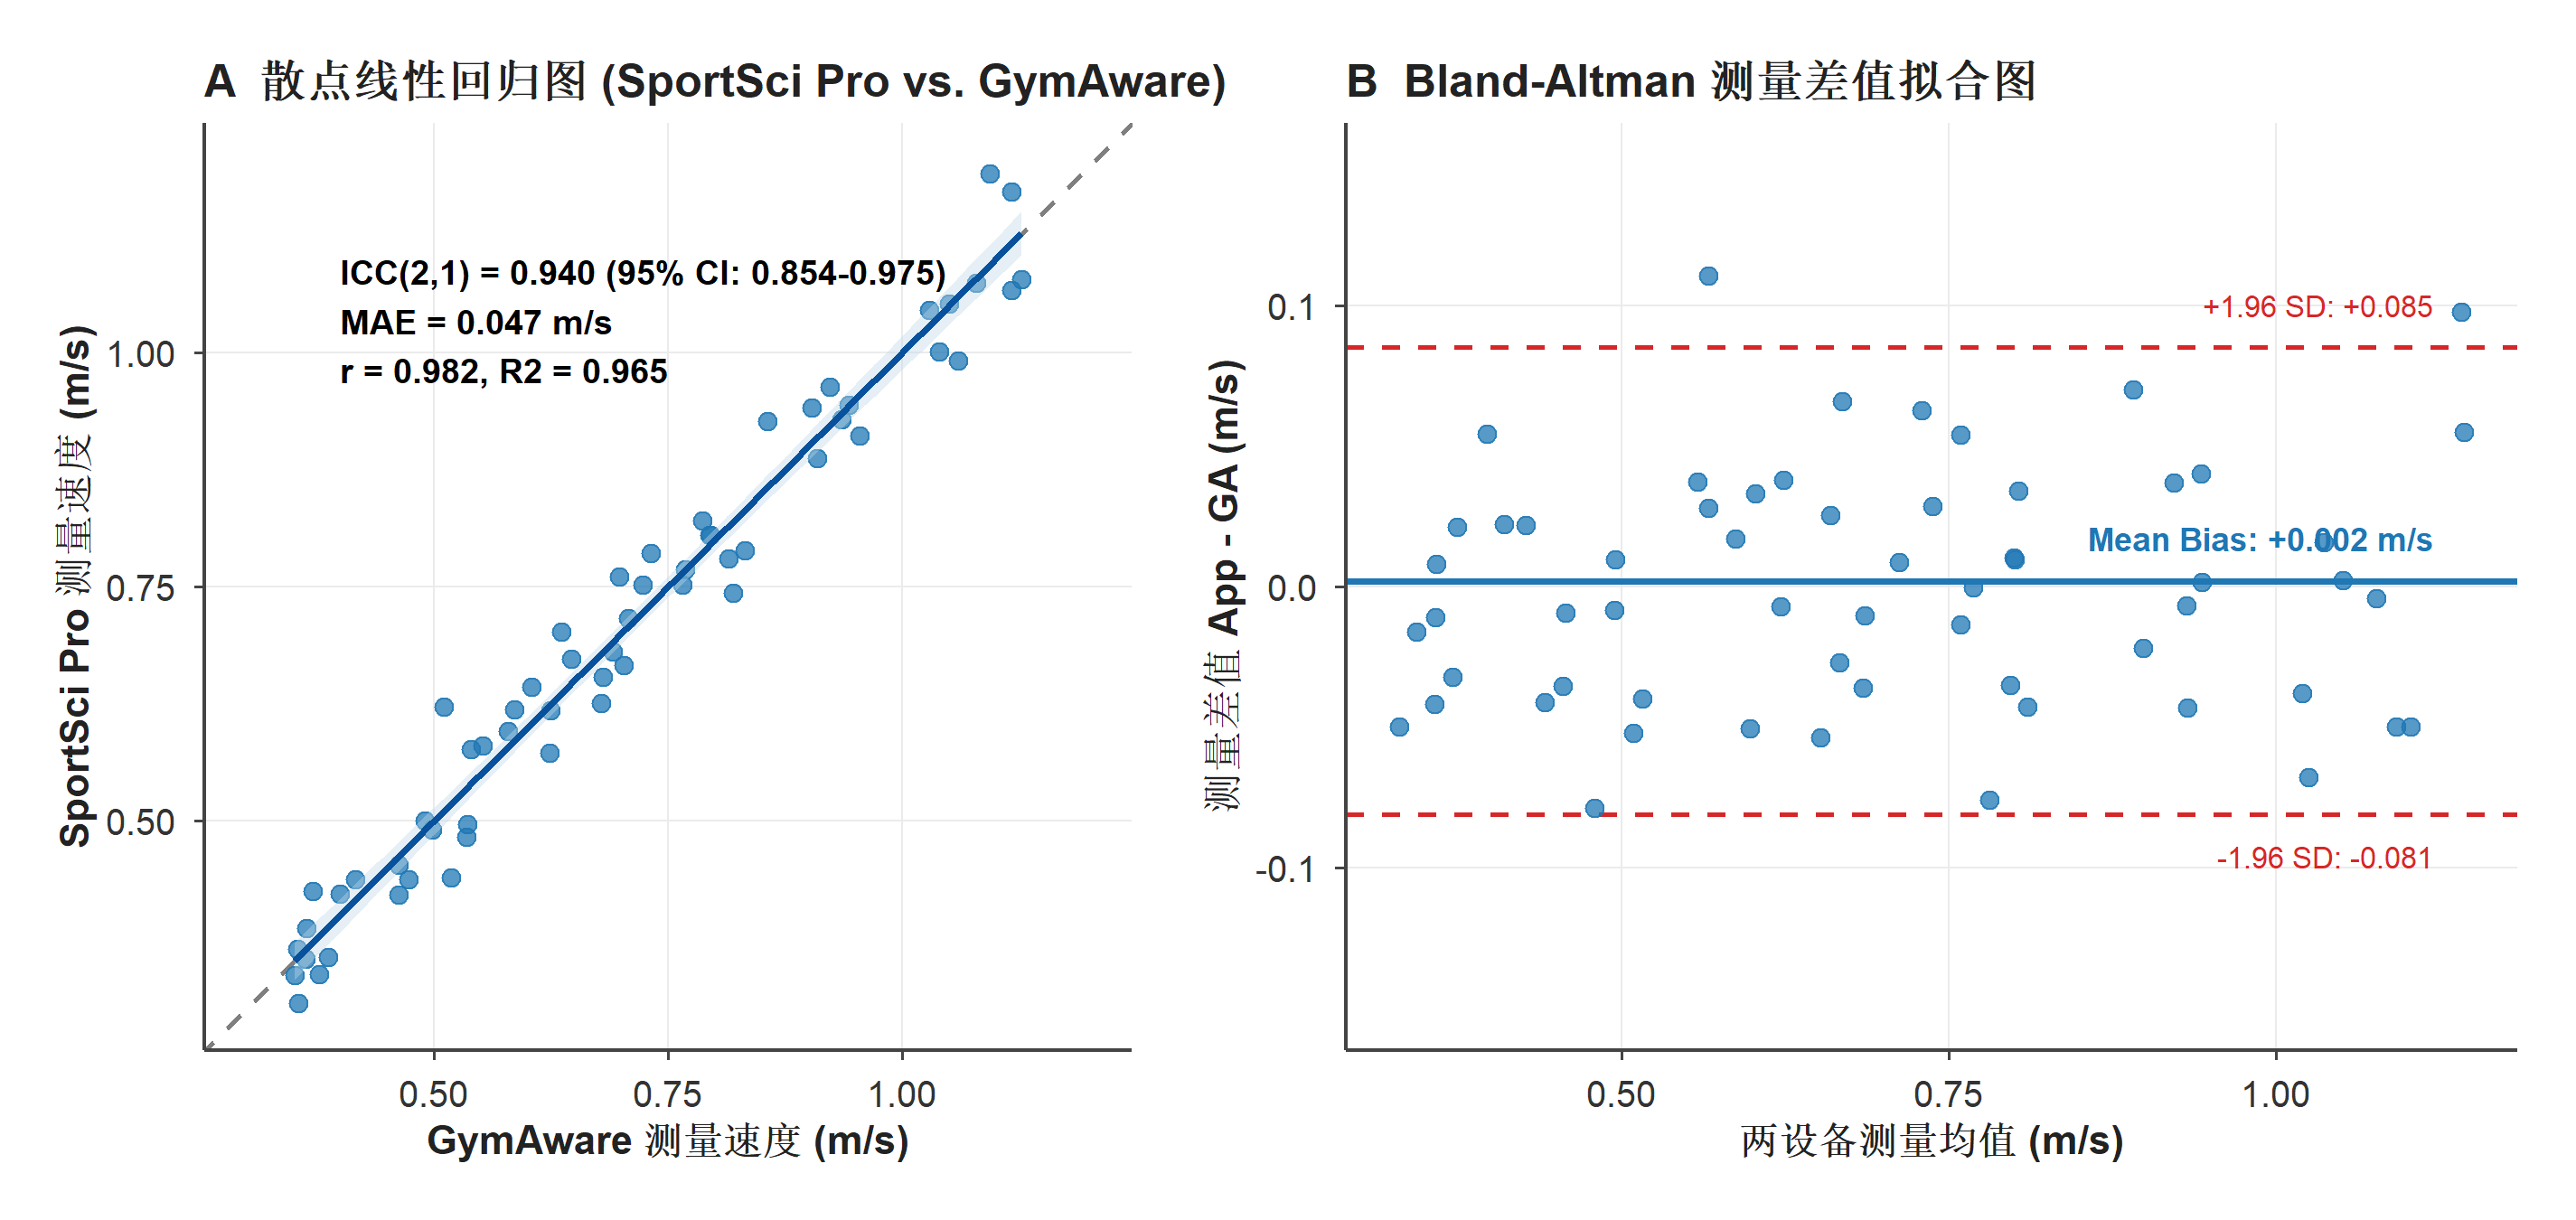
\includegraphics[width=0.95\textwidth]{figures/图4-2_研究一效度双子图.png}
\caption{A：散点线性回归图（SportSci Pro vs. GymAware），虚线为身份线，阴影为95\% CI；B：Bland-Altman测量差值图，红线为一致性界限}
\label{fig:validity_combined}
\end{figure}

\section{SportSci Pro真实训练场景生态效度补充分析}
\label{sec:ecological_validity}

研究二在干预期间以静默模式对AI辅助组受试者的训练课进行SportSci Pro与GymAware的同步记录, 用于评估研究一实验室效度结论在真实训练场景中的表现, 结果汇总见表~\ref{tab:validity_field}。

深蹲工作组Rep级配对分析共纳入43对有效配对样本（来自P006、P016、P025三名受试者）, ICC(2,1)=0.991（bootstrap 95\% CI：0.939至0.992）, 平均偏差Bias=+0.0019 m/s, MAE=0.017 m/s, 一致性界限（LoA）为$-$0.034至+0.038 m/s。

热身课次级配对分析共纳入88对有效配对样本（来自AI辅助组全部11名受试者）, ICC(2,1)=0.987（bootstrap 95\% CI：0.979至0.991）, Pearson相关系数$r$=0.9997。Bland-Altman分析显示Bias=+0.0212 m/s, LoA为+0.013至+0.030 m/s；88对配对中100\%均呈现App高于GymAware的正向偏差, 无一对呈现零偏移或负偏移。

现场生态效度Bland-Altman双子图分析结果见图~\ref{fig:ba_combined}。

\begin{figure}[htbp]
\centering
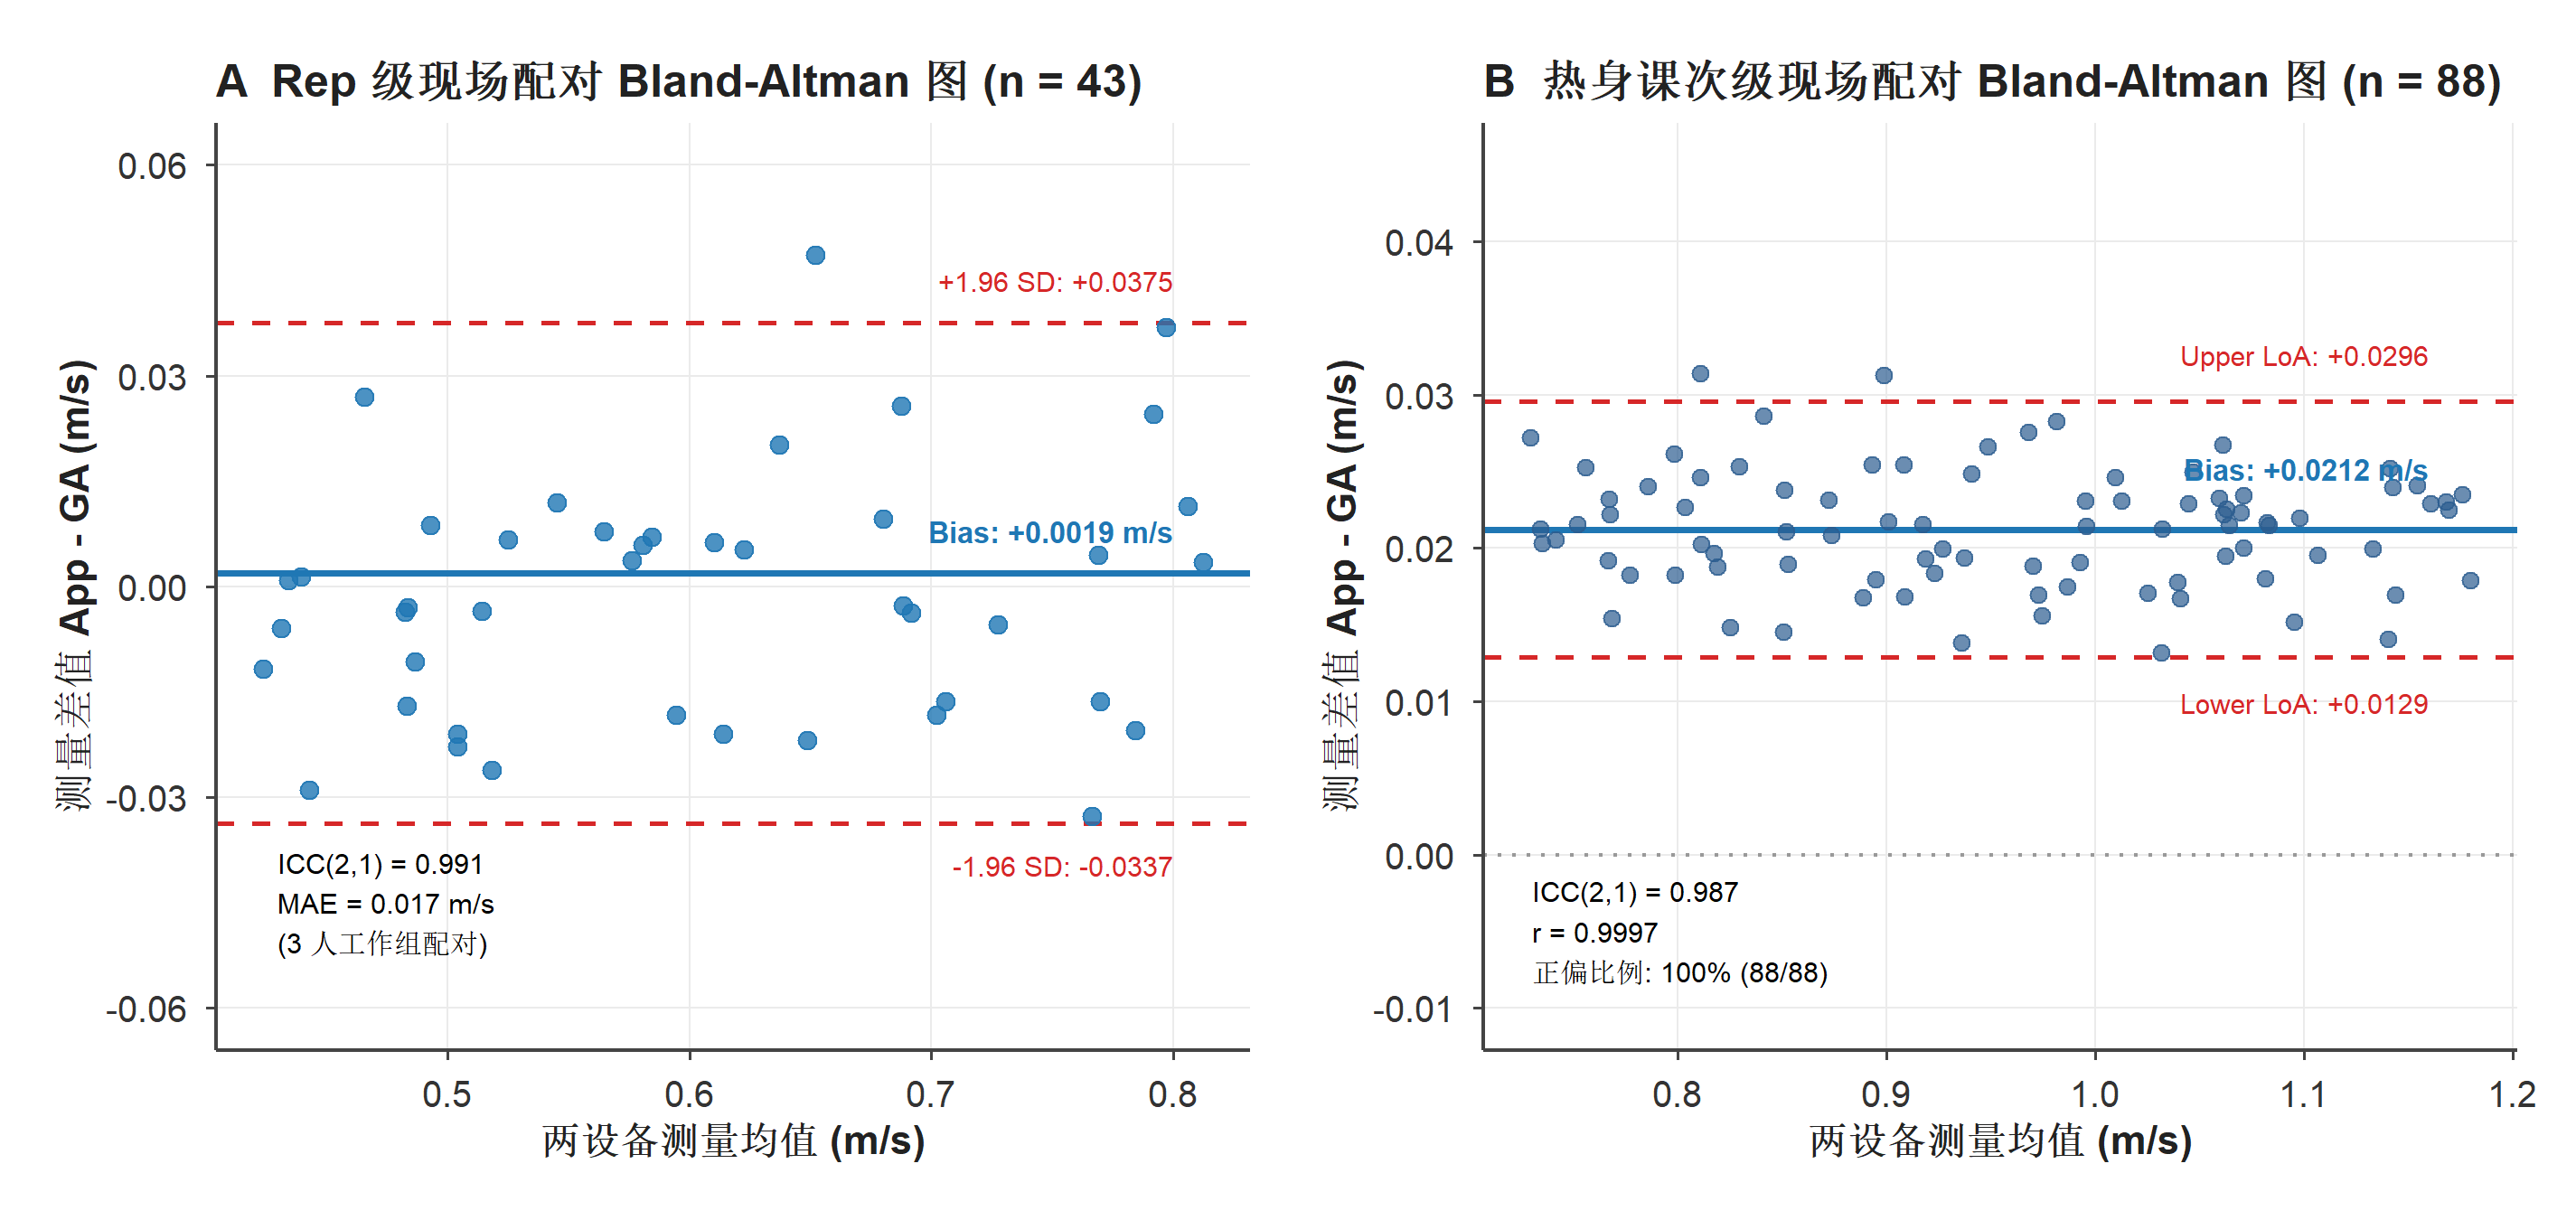
\includegraphics[width=0.9\textwidth]{figures/图4-4_现场生态效度Bland-Altman双子图.png}
\caption{A：深蹲工作组Rep级Bland-Altman分析（n=43对）；B：热身课次级现场配对Bland-Altman分析（n=88对）}
\label{fig:ba_combined}
\end{figure}

\begin{table}[htbp]
\centering
\caption{SportSci Pro与GymAware现场配对效度分析结果汇总表}
\label{tab:validity_field}
\zihao{5}
\begin{threeparttable}
\begin{tabular}{p{3.2cm}cc}
\toprule
\textbf{效度指标} & \textbf{Rep 级} & \textbf{热身级} \\
 & \textbf{（n = 43，3 人）} & \textbf{（n = 88，11 人）} \\
\midrule
ICC(2,1) & 0.991 & 0.987 \\
ICC 95\% CI（bootstrap） & (0.939, 0.992) & (0.979, 0.991) \\
Bias（m/s） & +0.0019 & +0.0212 \\
95\% LoA（m/s） & ($-$0.034, +0.038) & (+0.013, +0.030) \\
MAE（m/s） & 0.017 & 0.021 \\
Pearson $r$ & 0.991 & 0.9997 \\
正偏比例 & --- & 100\%（88/88 对） \\
\bottomrule
\end{tabular}
\begin{tablenotes}[flushleft]\footnotesize
\item 注：ICC 95\% CI 采用受试者级整簇 bootstrap 重抽样（10000 次）估计；LoA = 一致性界限（Limits of Agreement）；MAE = 平均绝对误差。
\end{tablenotes}
\end{threeparttable}
\end{table}

\section{研究二受试者流程与基线均衡性}
\label{sec:subject_flow}

研究二采用两组平行、开放标签随机对照预试验设计, 完整受试者流转情况遵循CONSORT-Pilot报告规范呈现。

\subsection{受试者流程}
\label{sec:consort_flow}

研究二通过便利招募方式共招募45名符合初筛条件的志愿者, 经知情同意与纳入排除标准核查后, 36名受试者完成签署知情同意书并进入随机化阶段。以基线相对深蹲最大力量（中位数分层）作为分层变量, 将36名受试者按1:1比例分配至AI辅助组（18人）与自我指导组（18人）。

随机化后, T0基线测试阶段共7名受试者脱落：AI辅助组4人（含1名基线测试期间发生腰部轻度肌肉拉伤退出的P028；其余3名因个人事务退出）, 自我指导组3人（均为个人事务退出）。上述T0期脱落者未进入正式干预阶段。

进入正式干预的29名受试者（AI辅助组14人, 自我指导组15人）在4周干预期间又有5名脱落：AI辅助组3人（含1名于第2周主动要求退出的P008与2名因出勤率不足被移出者）, 自我指导组2人（均为出勤率不足）。全部12名脱落者（T0期7人+干预期5人）均无T1后测数据, 不进入任何分析集。

最终24名受试者（AI辅助组11人, 自我指导组13人）完成T1后测并纳入符合方案集（PP）分析, 随机化后主要后测完成率为66.7\%（24/36）。

受试者完整流转情况见图~\ref{fig:consort}。

\begin{figure}[htbp]
\centering
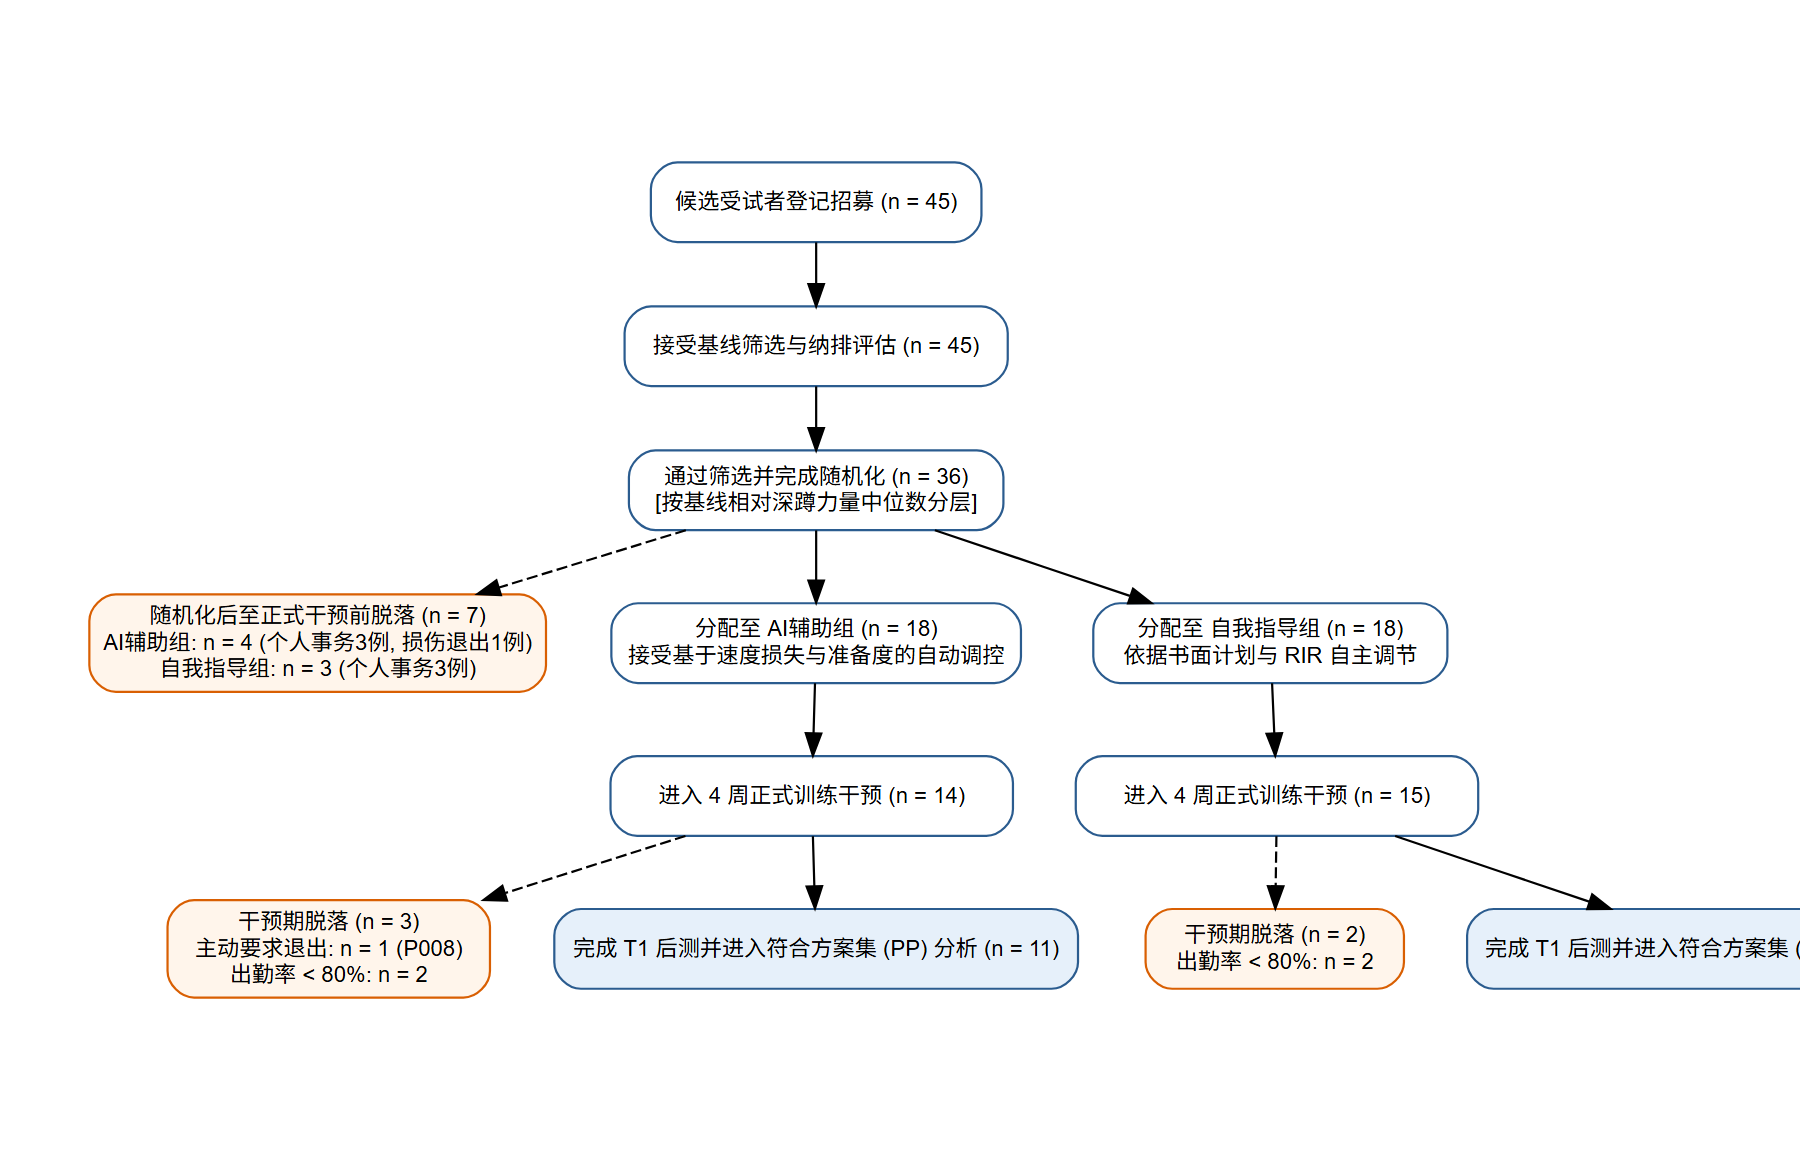
\includegraphics[width=0.8\textwidth]{figures/图4-1_CONSORT流程图.png}
\caption{研究二受试者CONSORT流程图}
\label{fig:consort}
\end{figure}

\subsection{基线特征均衡性}
\label{sec:baseline}

两组PP样本基线特征比较见表~\ref{tab:baseline_simplified}。12项连续基线指标的Welch独立样本$t$检验与Mann-Whitney U检验$p$值均大于0.05。作为分层变量的基线相对1RM在两组间高度接近：AI辅助组1.70$\pm$0.19 kg/kg, 自我指导组1.76$\pm$0.23 kg/kg, 组间差值$-$0.06 kg/kg（$p$=0.492, Hedges'$g$=$-$0.27）。

分类变量方面, Fisher确切检验显示：力量分层$p$=1.000（完全平衡）, 抗阻训练年限$p$=0.059, 每周训练频率$p$=0.027。后两项变量未纳入后续ANCOVA协变量调整。

\begin{table}[htbp]
\centering
\caption{研究二 PP 样本基线特征比较表（精简版，n = 24）}
\label{tab:baseline_simplified}
\zihao{5}
\begin{threeparttable}
\begin{tabular}{p{3.0cm}ccc>{\raggedleft\arraybackslash}p{1.5cm}}
\toprule
\textbf{变量} & \textbf{AI 组} & \textbf{Self 组} & \textbf{p 值} & \textbf{Hedges' g} \\
 & \textbf{（n = 11）} & \textbf{（n = 13）} & & \\
\midrule
年龄（岁）              & 24.91 $\pm$ 2.55     & 23.85 $\pm$ 1.63     & 0.250 & 0.49 \\
身高（cm）              & 179.73 $\pm$ 7.13    & 176.00 $\pm$ 4.58    & 0.154 & 0.61 \\
体重（kg）              & 77.54 $\pm$ 10.20    & 74.27 $\pm$ 4.79     & 0.346 & 0.41 \\
基线深蹲 1RM（kg）      & 130.68 $\pm$ 12.15   & 130.77 $\pm$ 17.45   & 0.989 & --0.01 \\
基线相对 1RM（kg/kg）   & 1.70 $\pm$ 0.19      & 1.76 $\pm$ 0.23      & 0.492 & --0.27 \\
基线 CMJ（cm）          & 59.66 $\pm$ 5.23     & 60.52 $\pm$ 6.27     & 0.720 & --0.14 \\
基线训练自我效能（分）  & 65.45 $\pm$ 5.09     & 65.69 $\pm$ 6.91     & 0.924 & --0.04 \\
\bottomrule
\end{tabular}
\begin{tablenotes}[flushleft]\footnotesize
\item 注：连续变量以均值 $\pm$ 标准差表示；组间比较采用 Welch 独立样本 t 检验，全部变量 p 值均 $>$ 0.05；分层变量基线相对 1RM 组间差异极小（g = --0.27），证实分层随机化程序有效。完整 12 项基线变量（含 BMI、体脂率、骨骼肌量、去脂体重、基线 SJ 及双检验 p 值等）见附录 A 附表 A-1。
\end{tablenotes}
\end{threeparttable}
\end{table}

\section{可行性、训练完成情况与推进标准对照}
\label{sec:feasibility}

研究二在招募保留、训练执行与系统操作三个维度评估了方案的可行性, 并对照预设推进标准进行判定。

\subsection{招募与保留}
\label{sec:recruitment}

研究二从45名报名者中, 36名完成随机化（随机化率80.0\%）, 29名进入干预（进入干预率29/36=80.6\%）, 24名完成主要后测（主要后测完成率66.7\%）。12名脱落者中, 7名（58.3\%）发生于随机化后至正式干预开始前的T0基线测试过渡阶段, 5名（41.7\%）发生于4周干预期间。

\subsection{训练执行}
\label{sec:training_execution}

PP样本24名受试者在4周干预期间共执行192个训练课次, 其中189个课次完成了完整的过程记录（训练完成率189/192=98.4\%）, 3个课次因关键字段缺失未达到完整记录标准（P001缺S3, P005缺S1, P010缺S6, 均为AI辅助组）。24名PP受试者均达到$\geq$80\%课次的高依从标准（100\%, 24/24）。

\subsection{AI辅助组执行质量}
\label{sec:ai_execution}

AI辅助组11名受试者的速度目标命中率均值为80.2\%$\pm$6.9\%, 个体范围69.0\%--89.5\%, 全部11人均达到$\geq$60\%预设标准。自动减组规则共有3名受试者触发, 累计4次：P009在S1触发1次（因Readiness CMJ低于基线95\%阈值）、P010在S1触发1次（同样为Readiness不足）、P016在S4与S6各触发1次共2次。\allowbreak 自动减组规则的触发逻辑与降组建议执行忠实度为100\%。

\subsection{安全性}
\label{sec:safety}

研究期间未发生严重不良事件（SAE 0例）。非严重不良事件1例：P028在T0基线测试期发生腰部轻度肌肉拉伤, 未就医治疗, 随后自愿退出研究。

\subsection{推进标准综合对照}
\label{sec:criteria}

上述指标与预设推进标准的对照汇总见表~\ref{tab:progression_criteria}。9项预设指标中, 7项达标, 2项未达标（主要后测完成率66.7\%、AI辅助组SUS评分65.00分）。\allowbreak

\begin{table}[htbp]
\centering
\caption{研究二可行性指标与预设推进标准对照表}
\label{tab:progression_criteria}
\zihao{5}
\begin{threeparttable}
\begin{tabular}{@{}llccc@{}}
\toprule
\textbf{评估维度} & \textbf{指标} & \textbf{预设阈值} & \textbf{实际结果} & \textbf{判定} \\
\midrule
招募可行性 & 进入干预率           & $\ge$ 80\%   & 29/36（80.6\%）    & 临界达标 \\
招募保留   & 主要后测完成率       & $\ge$ 80\%   & 24/36（66.7\%）    & \textbf{未达标} \\
方案依从性 & 训练完成率           & $\ge$ 80\%   & 189/192（98.4\%）  & 达标 \\
方案依从性 & 高依从率（$\ge$ 80\% 课次） & $\ge$ 80\% & 24/24（100.0\%）   & 达标 \\
数据质量   & 数据完整性（PP 层）  & $\ge$ 90\%   & 100.0\%            & 达标 \\
系统体验   & AI 辅助组 SUS 评分   & $\ge$ 70 分  & 65.00 $\pm$ 4.61    & \textbf{未达标} \\
过程控制   & 速度目标命中率       & $\ge$ 60\%   & 80.2\% $\pm$ 6.9\%  & 达标 \\
算法执行   & 自动减组忠实度       & 无系统异常   & 100\%（4/4 次）    & 达标 \\
安全性     & 严重不良事件         & 0 例         & 0 例               & 达标 \\
\bottomrule
\end{tabular}
\begin{tablenotes}[flushleft]\footnotesize
\item 注：9 项预设推进标准中，7 项达标（含 1 项临界达标），2 项未达标（主要后测完成率与 AI 辅助组 SUS 评分）。
\end{tablenotes}
\end{threeparttable}
\end{table}

\section{两组训练执行与负荷结构}
\label{sec:training_execution_results}

两组在4周共8次训练中累积的外部训练负荷、内部负荷反应与派生结构指标的组间比较结果见表~\ref{tab:training_execution}.

\begin{table}[htbp]
\centering
\caption{两组训练执行指标 Welch $t$ 检验结果汇总表}
\label{tab:training_execution}
\zihao{5}
\begin{threeparttable}
\begin{tabular}{p{3.2cm}ccc>{\raggedleft\arraybackslash}p{1.3cm}c}
\toprule
\textbf{变量} & \textbf{AI 组} & \textbf{Self 组} & \textbf{差值} & \textbf{p} & \textbf{Hedges' g} \\
 & \textbf{（n = 11）} & \textbf{（n = 13）} & & & \\
\midrule
全期总负荷（kg）             & 17651.8 $\pm$ 2198.6 & 17461.5 $\pm$ 2792.1 & +190.28 & 0.854 & 0.07 \\
深蹲主项总负荷（kg）         & 13654.5 $\pm$ 1819.3 & 13642.3 $\pm$ 2226.5 & +12.24  & 0.988 & 0.01 \\
平均每课次负荷（kg）         & 2297.7 $\pm$ 370.7   & 2182.7 $\pm$ 349.0   & +115.05 & 0.445 & 0.31 \\
总组数                       & 28.2 $\pm$ 1.6       & 29.1 $\pm$ 1.1       & --0.90  & 0.136 & --0.64 \\
\textbf{总完成重复次数}       & \textbf{100.3 $\pm$ 6.5} & \textbf{105.5 $\pm$ 4.1} & \textbf{--5.19} & \textbf{0.035*} & \textbf{--0.95} \\
全期平均 sRPE（0--10 分）    & 6.5 $\pm$ 0.5        & 6.4 $\pm$ 0.3        & +0.06   & 0.735 & 0.14 \\
训练总时长（min）            & 822.7 $\pm$ 26.2     & 798.8 $\pm$ 35.5     & +23.88  & 0.072 & 0.73 \\
个体 Hooper 均值（分）       & 20.4 $\pm$ 2.5       & 19.8 $\pm$ 1.1       & +0.62   & 0.453 & 0.33 \\
\bottomrule
\end{tabular}
\begin{tablenotes}[flushleft]\footnotesize
\item 注：\textbf{* p $<$ 0.05}。派生指标"每次重复平均负荷" = 深蹲主项总负荷 $\div$ 总重复次数（AI 辅助组约 136.7 kg/rep；自我指导组约 128.9 kg/rep；差值约 +6.1\%）。
\end{tablenotes}
\end{threeparttable}
\end{table}

两组在全期总外部负荷（$p$=0.854）、深蹲主项总负荷（$p$=0.988）、全期平均sRPE（$p$=0.735）与个体Hooper均值（$p$=0.453）上均未表现出统计学差异。

在负荷组织形态上, 自我指导组完成的总重复次数显著高于AI辅助组（105.5$\pm$4.1 vs. 100.3$\pm$6.5次, $p$=0.035）。派生指标计算显示, AI辅助组每次重复的平均外部负荷约为136.7 kg/rep, 自我指导组约为128.9 kg/rep, 差值约+6.1\%（派生自深蹲总负荷$\div$总重复次数）。AI辅助组的单次训练时长平均比自我指导组多约24分钟（822.7 vs. 798.8 min, $p$=0.072）。

\section{Hooper主观恢复状态的训练过程动态}
\label{sec:hooper}

采用线性混合效应模型（LMM）对8次训练课前的Hooper主观恢复总分进行纵向分析。模型设定为：\texttt{Hooper\_final $\sim$ Group $\times$ Sess\_factor + (1|ID)}, 采用Kenward-Roger Type III F检验进行固定效应显著性推断（表~\ref{tab:hooper_lmm}）。

\begin{table}[htbp]
\centering
\caption{Hooper 主观恢复线性混合效应模型 Type III 方差分析表（Kenward-Roger）}
\label{tab:hooper_lmm}
\zihao{5}
\begin{threeparttable}
\begin{tabular}{@{}lcccc@{}}
\toprule
\textbf{变异来源} & \textbf{F 值} & \textbf{NumDF} & \textbf{DenDF} & \textbf{p 值} \\
\midrule
组别（Group）              & 0.67 & 1 & 22.0  & 0.421 \\
课次（Session）            & \textbf{3.09} & \textbf{7} & \textbf{154.0} & \textbf{0.004**} \\
组别 $\times$ 课次（交互）  & 0.32 & 7 & 154.0 & 0.945 \\
\bottomrule
\end{tabular}
\begin{tablenotes}[flushleft]\footnotesize
\item 注：\textbf{** p $<$ 0.01}。模型设定为 Hooper\_final $\sim$ Group $\times$ Sess\_factor $+$ (1$\vert$ID)，采用 Kenward-Roger 自由度修正。跨全部课次的组间边际均值差为 +0.62 分（95\% CI：--0.95 至 2.20），全部 8 个课次的差值 95\% CI 均跨越无效值 0。
\end{tablenotes}
\end{threeparttable}
\end{table}

组别主效应不显著（$F$(1, 22.0)=0.67, $p$=0.421）, 组别与课次交互效应不显著（$F$(7, 154.0)=0.32, $p$=0.945）, 课次主效应达到统计学显著（$F$(7, 154.0)=3.09, $p$=0.004）。

各课次组间差值的emmeans pairwise比较显示, 8个课次的AI辅助组$-$自我指导组差值范围为$-$0.16至+1.37分, 全部8个课次的差值95\%置信区间均跨越无效值0, 跨全部课次的组间边际均值差为+0.62分（95\% CI：$-$0.95至2.20）, BH校正后$p$值均在0.26至0.98之间。

从描述性统计层面观察各课次Hooper均值的时间演变, AI辅助组由S1的19.91分逐步上升至S4峰值21.45分, 随后在S8回落至18.45分；自我指导组由S1的18.54分逐步上升至S6峰值20.85分, 随后在S8回落至18.62分。本研究未对各课次之间的两两pairwise比较进行显著性检验, 因此上述时间演变形态属于对课次主效应显著（$p$=0.004）的形态学描述, 不构成对特定课次间差异的统计学推断。

各课次Hooper均值的时间演变趋势见图~\ref{fig:hooper_trend}。

\begin{figure}[htbp]
\centering
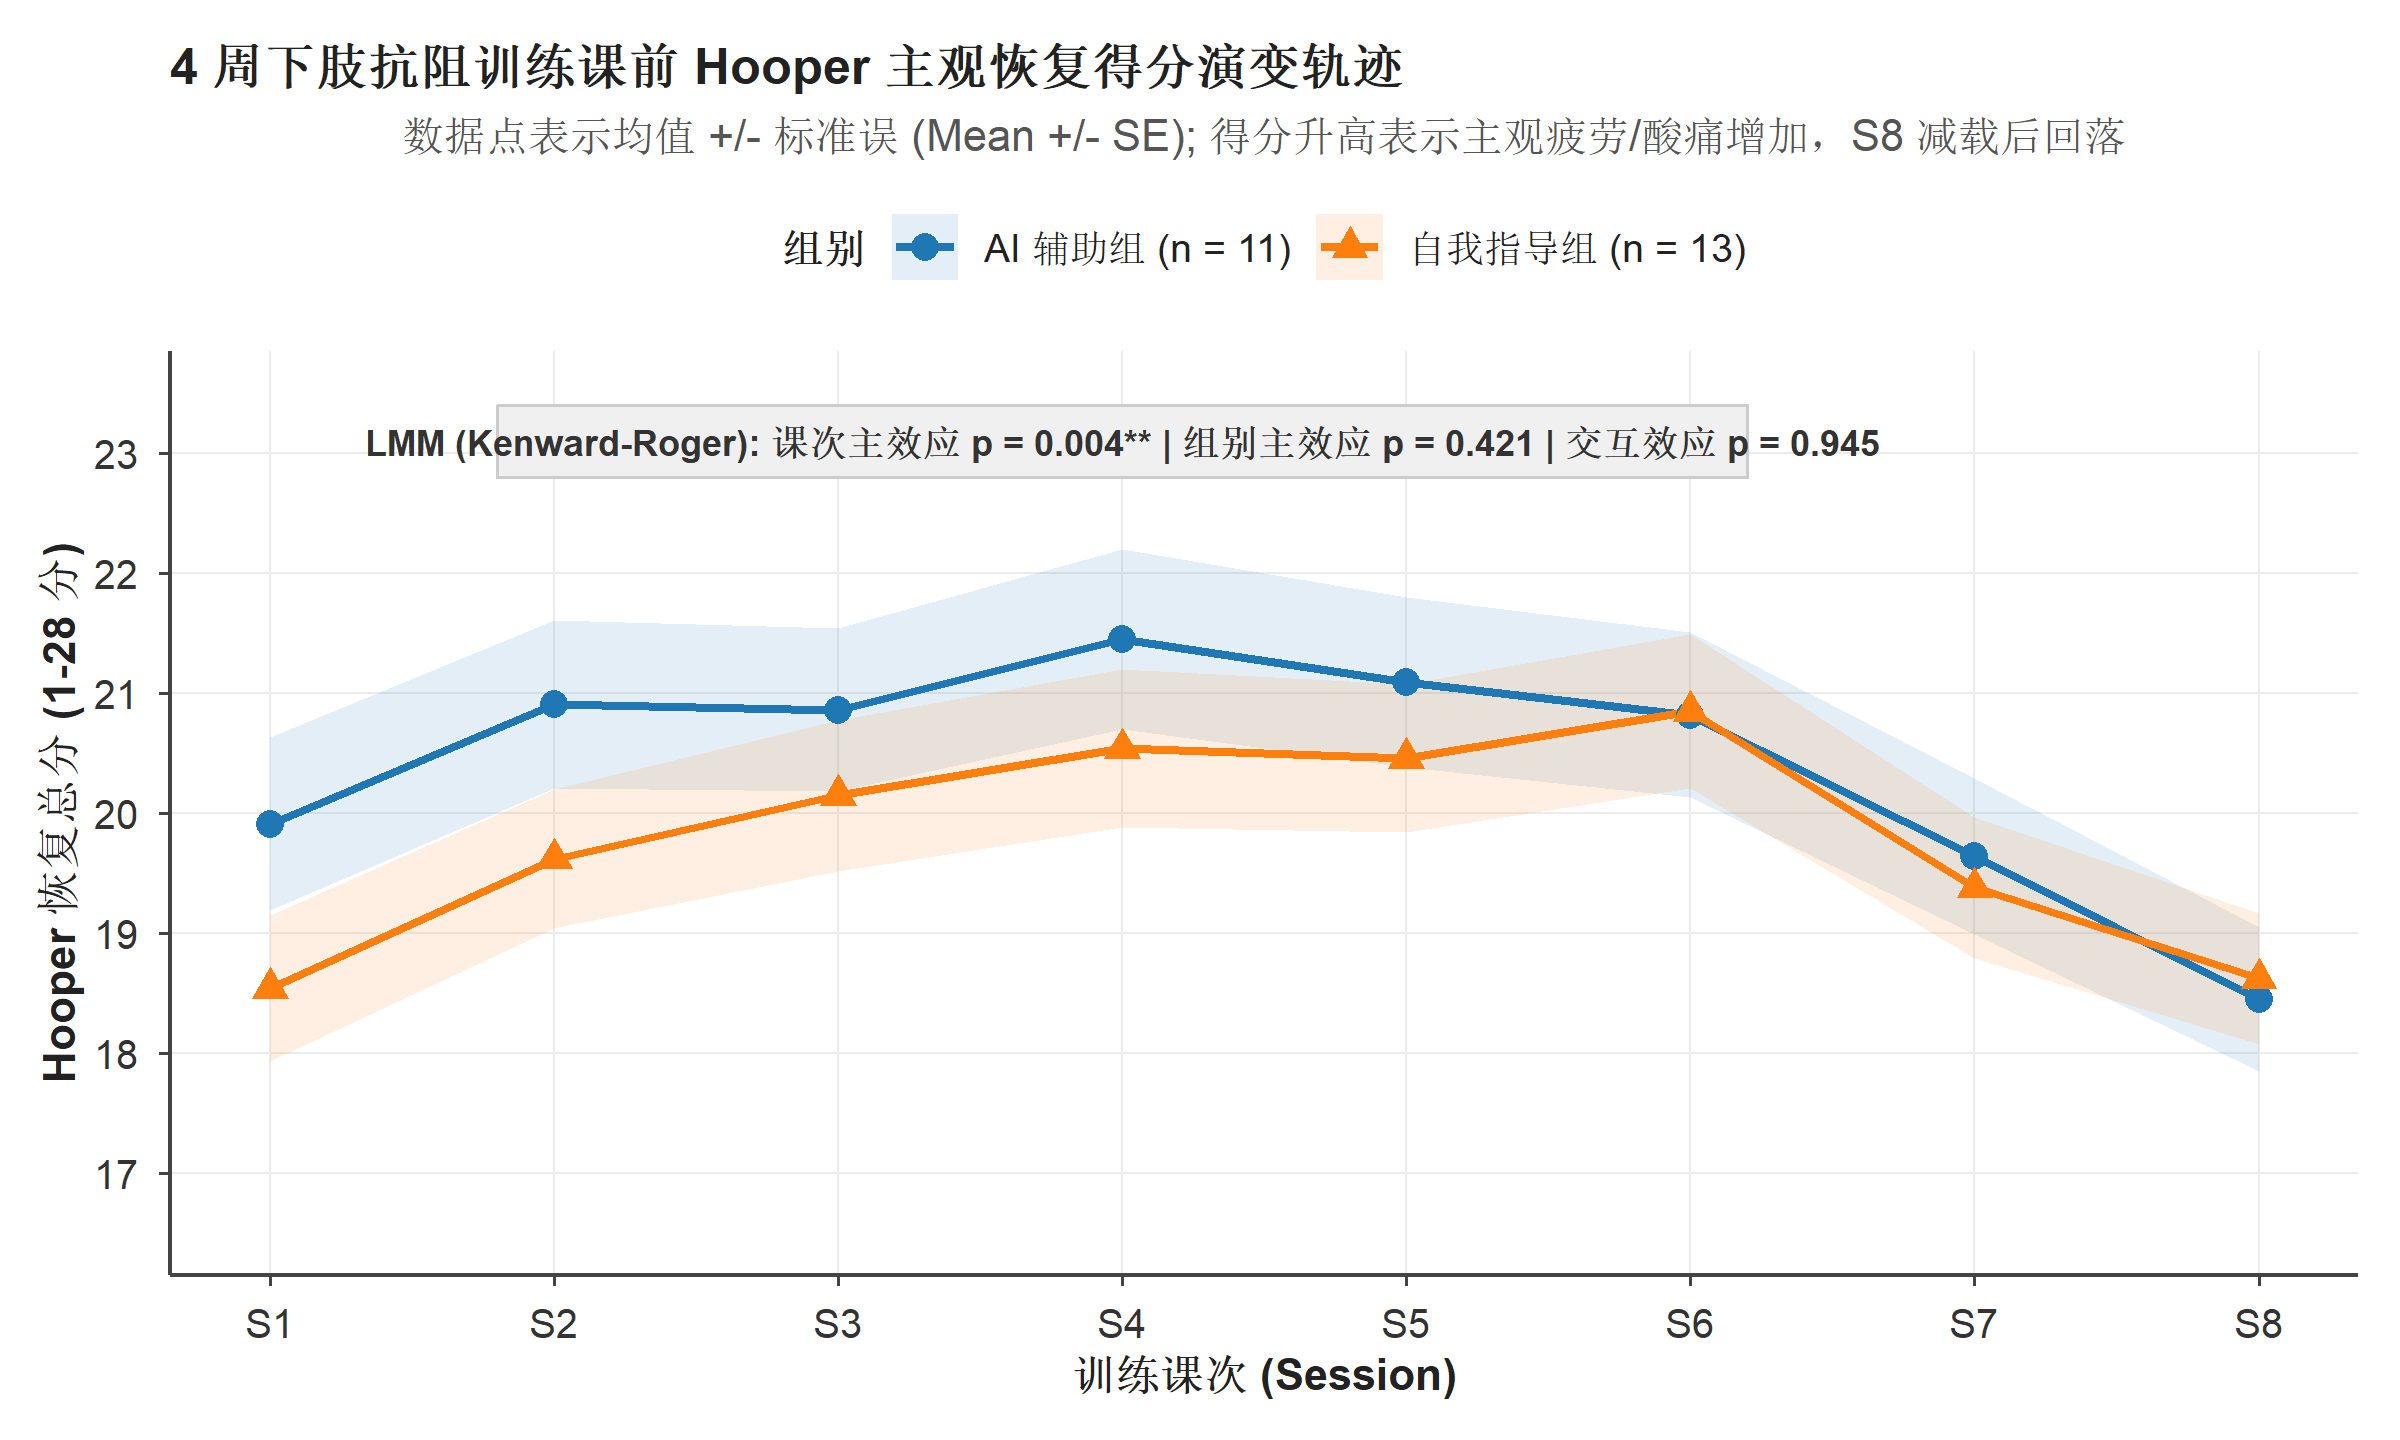
\includegraphics[width=0.85\textwidth]{figures/图4-3_Hooper_S1-S8趋势图.png}
\caption{两组8次训练课前Hooper主观恢复总分均值演变趋势；LMM Kenward-Roger检验结果：课次主效应 p = 0.004**，组别主效应 p = 0.421，交互效应 p = 0.945}
\label{fig:hooper_trend}
\end{figure}

\section{主要探索性体能与心理结局的组间比较}
\label{sec:ancova}

研究二将深蹲绝对1RM、深蹲相对1RM、CMJ高度、SJ高度和训练自我效能五项指标作为探索性适应结局, 采用协方差分析（ANCOVA）模型进行比较, 模型设定为\texttt{Post $\sim$ Group + Pre + Stratum}, 采用Type III偏差平方和进行组间效应估计。分析结果见表~\ref{tab:ancova_simplified}。

\begin{landscape}
\begin{table}[htbp]
\centering
\caption{探索性结局指标 ANCOVA 结果汇总表（精简版，n = 24）}
\label{tab:ancova_simplified}
\zihao{5}
\begin{threeparttable}
\begin{tabular}{@{}lcccc@{}}
\toprule
\textbf{结局指标} & \textbf{调整后差值（AI--Self）} & \textbf{p 值} & \textbf{Hedges' g} & \textbf{FDR 校正 p} \\
\midrule
深蹲绝对 1RM（kg）      & +2.43  & 0.266 & 0.46 & 0.341 \\
深蹲相对 1RM（kg/kg）   & +0.03  & 0.273 & 0.39 & 0.341 \\
CMJ 高度（cm）          & +2.16  & 0.051 & 0.85 & 0.126 \\
SJ 高度（cm）           & +0.39  & 0.622 & 0.43 & 0.622 \\
\textbf{训练自我效能（分）} & \textbf{+9.88} & \textbf{$<$0.001**} & \textbf{2.70} & \textbf{$<$0.001**} \\
\bottomrule
\end{tabular}
\begin{tablenotes}[flushleft]\footnotesize
\item 注：\textbf{** p $<$ 0.001}。ANCOVA 模型设定为 Post $\sim$ Group $+$ Pre $+$ Stratum，采用 Type III 偏差平方和。差值正值表示 AI 辅助组高于自我指导组；Hedges' g 为小样本校正效应量。完整结果表（含 T1 均值、差值 95\% CI、Hedges' g 95\% CI）见附录 A 附表 A-2。
\end{tablenotes}
\end{threeparttable}
\end{table}
\end{landscape}

在体能适应结局上, 深蹲绝对1RM（调整后差值+2.43 kg, $p$=0.266）、相对1RM（+0.03 kg/kg, $p$=0.273）与SJ高度（+0.39 cm, $p$=0.622）三项指标的差值95\% CI与Hedges'$g$的95\% CI均跨越无效值0。

在CMJ高度上, AI辅助组的调整后差值为+2.16 cm（$p$=0.051）：差值95\% CI为（$-$0.01, 4.33）, 下界近似零但未完全排除零效应；Hedges'$g$=0.85, $g$ 95\% CI为(0.02, 1.69), 下界略高于零。FDR校正后$p$=0.126。

在训练自我效能上, AI辅助组的调整后差值达+9.88分（$p<0.001$, Hedges'$g$=2.70）。基线时AI辅助组为65.45分, 自我指导组为65.69分；4周干预后AI辅助组升至83.18分（净增+17.73分）, 自我指导组升至73.69分（净增+8.00分）。该指标FDR校正后仍保持极显著水平。

五项探索性结局指标的标准化效应量及其95\% CI汇总见图~\ref{fig:forest}。

\begin{figure}[htbp]
\centering
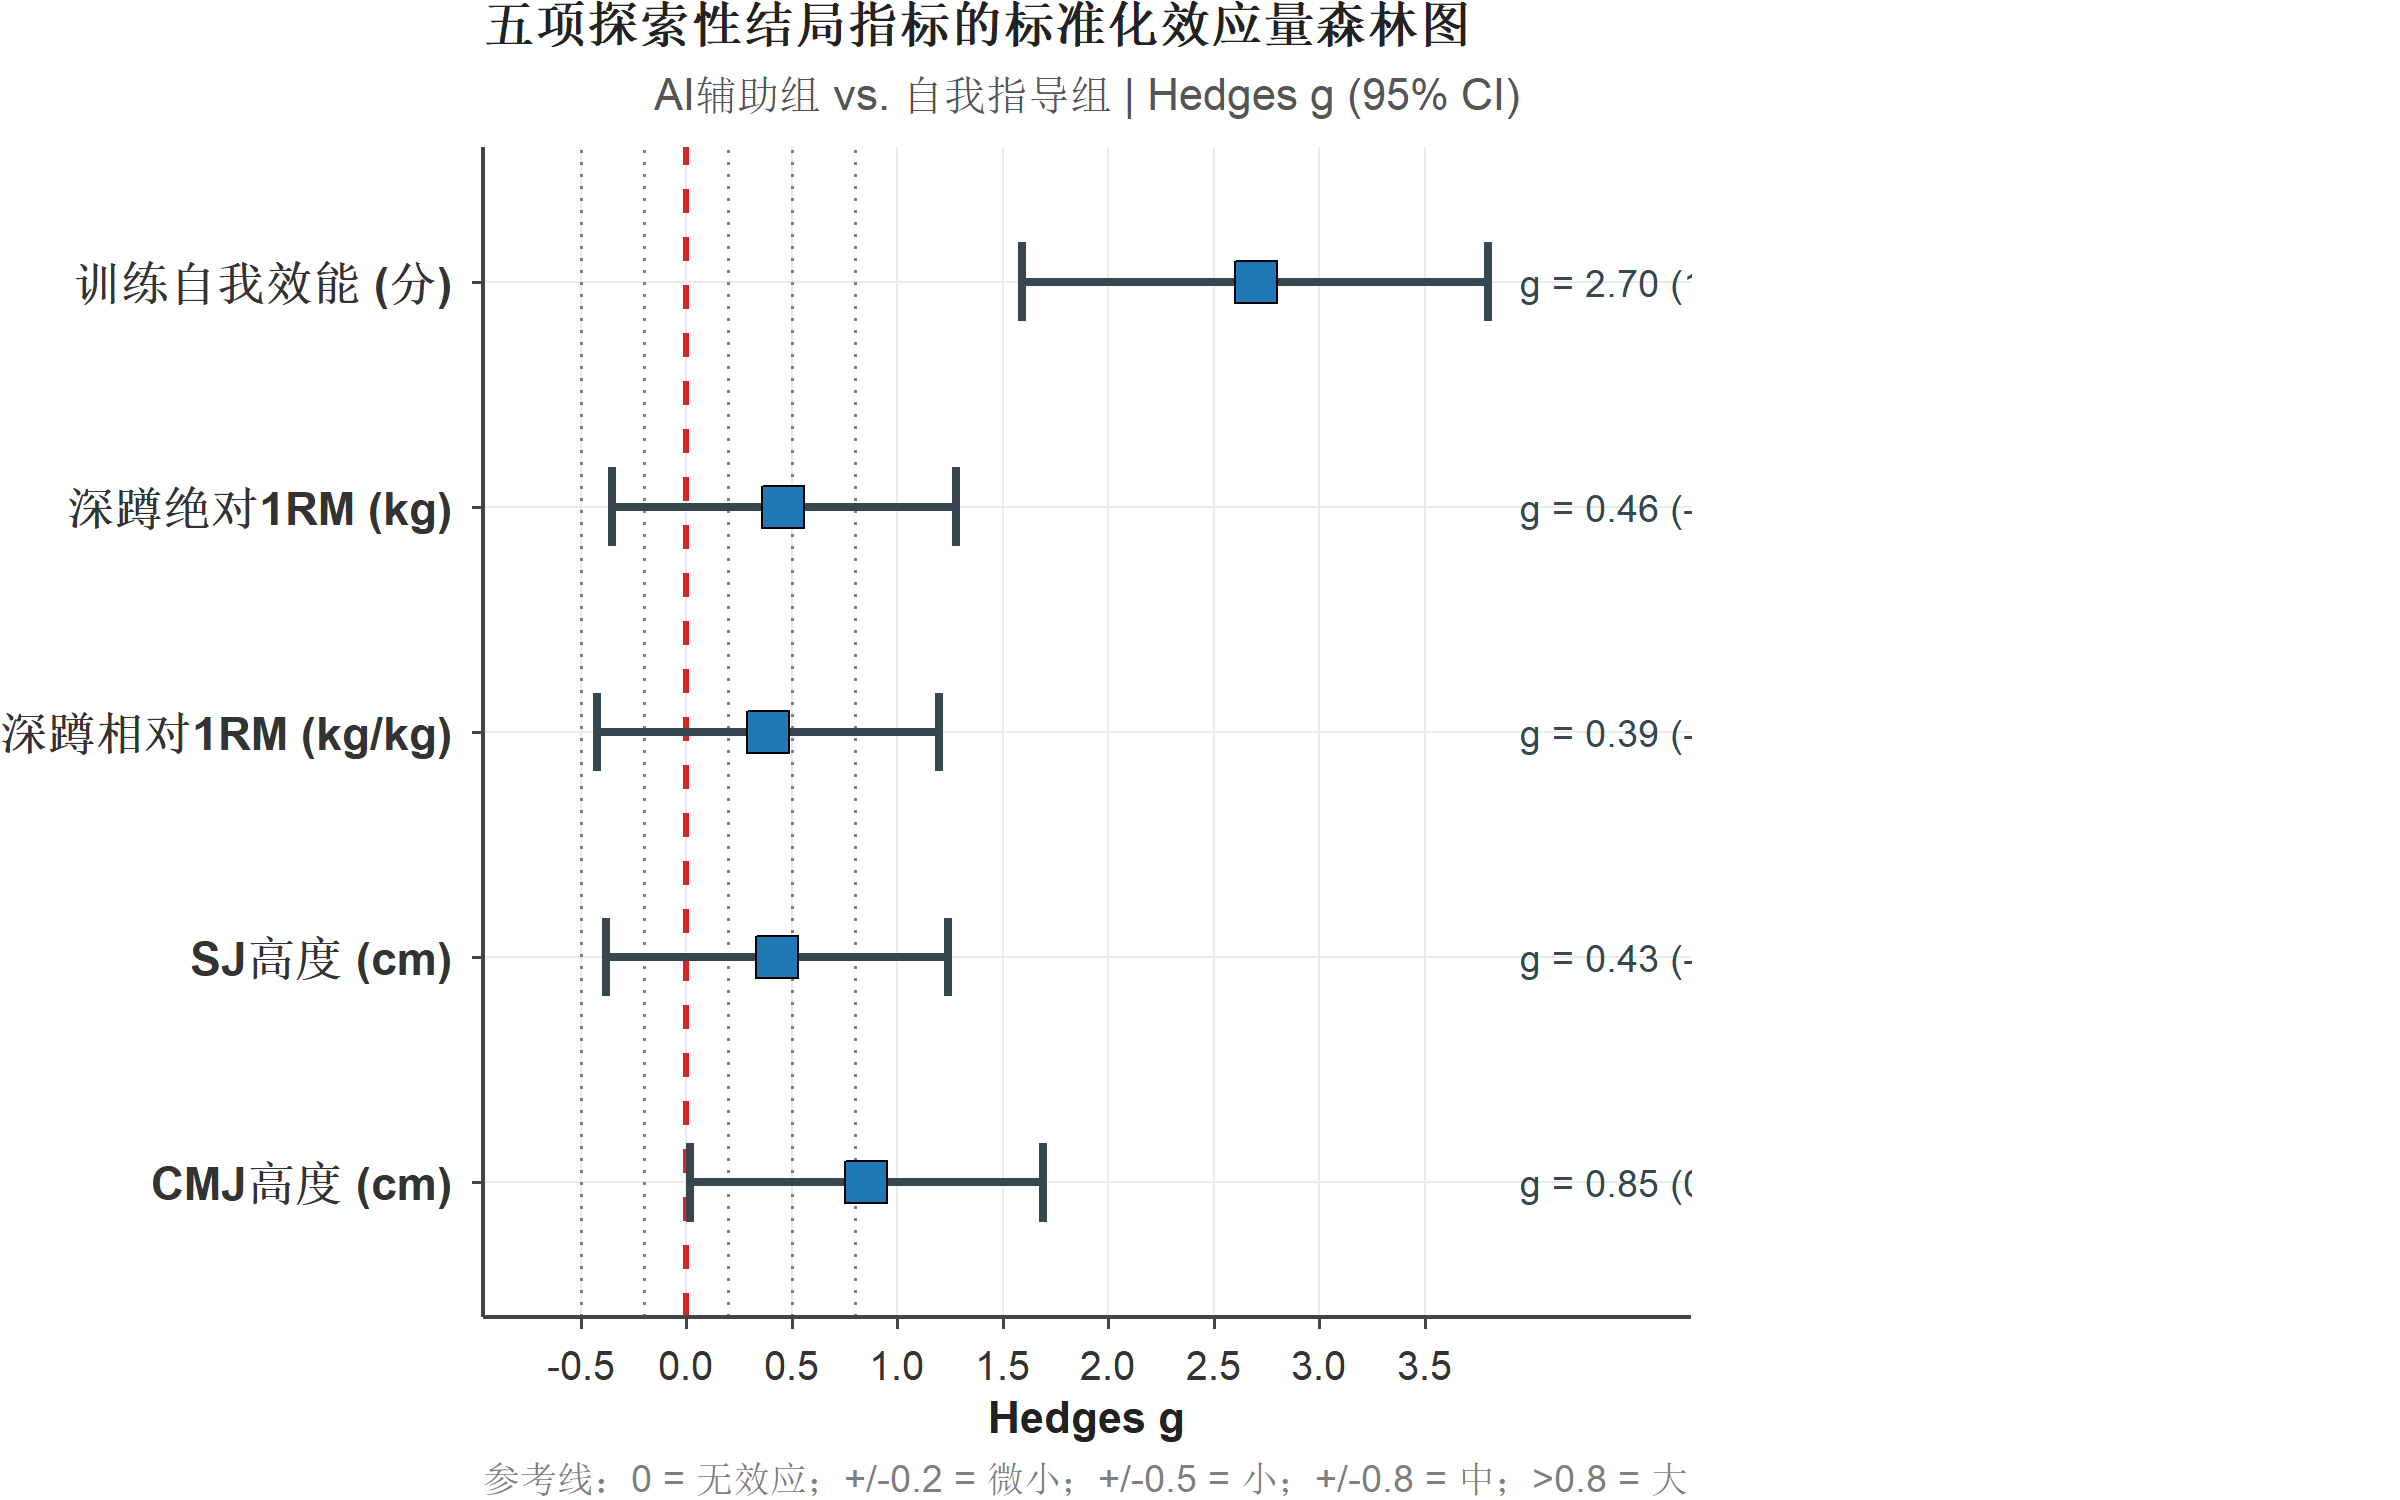
\includegraphics[width=0.85\textwidth]{figures/图4-6_五项主要结局森林图.png}
\caption{五项探索性结局指标标准化效应量森林图}
\label{fig:forest}
\end{figure}

\section{训练负荷与结局变化的探索性关联}
\label{sec:correlation}

研究二对训练执行变量与T1后测结局指标之间进行了探索性Spearman相关分析, 完整相关矩阵共包含28对变量组合。28对中, 原始显著性检验显示8对达到$p<0.05$的名义显著水平, 经Benjamini-Hochberg FDR校正后, 全部28对相关均未达到统计学显著（FDR校正后$p$均$>$0.05）。原始$p<0.05$的8对相关汇总见表~\ref{tab:spearman}。

\begin{table}[htbp]
\centering
\caption{训练负荷与结局变化的探索性 Spearman 相关（原始 p $<$ 0.05 组合）}
\label{tab:spearman}
\zihao{5}
\begin{threeparttable}
\begin{tabular}{@{}llccc@{}}
\toprule
\textbf{训练执行变量} & \textbf{结局变量} & \textbf{Spearman $\rho$} & \textbf{原始 p 值} & \textbf{FDR 校正 p 值} \\
\midrule
训练总时长        & $\Delta$绝对 1RM & +0.533 & 0.007 & 0.093 \\
平均每课次负荷    & $\Delta$绝对 1RM & +0.500 & 0.013 & 0.093 \\
全期总负荷        & $\Delta$绝对 1RM & +0.441 & 0.031 & 0.108 \\
个体 Hooper 均值  & $\Delta$绝对 1RM & --0.455 & 0.025 & 0.102 \\
总次数            & $\Delta$SJ       & +0.503 & 0.012 & 0.093 \\
总组数            & $\Delta$SJ       & +0.479 & 0.018 & 0.093 \\
训练总时长        & $\Delta$SJ       & +0.494 & 0.014 & 0.093 \\
全期平均 sRPE     & $\Delta$SJ       & --0.472 & 0.020 & 0.093 \\
\bottomrule
\end{tabular}
\begin{tablenotes}[flushleft]\footnotesize
\item 注：完整 28 对相关矩阵详见附录 B 附表 B-2。经 Benjamini-Hochberg FDR 校正后，全部 28 对相关均未达到统计学显著（校正后 p 均 $>$ 0.05）。
\end{tablenotes}
\end{threeparttable}
\end{table}

在方向性观察层面, 训练总时长、平均每课次负荷与全期总负荷均与$\Delta$绝对1RM呈中等正相关（$\rho$范围+0.441至+0.533）, 个体Hooper均值与$\Delta$绝对1RM呈中等负相关（$\rho$=$-$0.455）；总次数、总组数与训练总时长均与$\Delta$SJ呈中等正相关（$\rho$范围+0.479至+0.503）, 全期平均sRPE与$\Delta$SJ呈中等负相关（$\rho$=$-$0.472）。

\section{研究三质性访谈结果}
\label{sec:study3_qualitative}

研究三采用半结构化深度访谈, 对12名完成干预的受试者（AI辅助组5人, 自我指导组7人）进行了一对一访谈, 采用三轮主题分析法进行资料分析。经选择性编码后, 提炼出核心范畴与六大主题。

\subsection{核心范畴}

\textbf{训练者如何在客观反馈与自主判断之间协商训练决策。}

该核心范畴能够同时整合AI辅助组和自我指导组资料：AI辅助组主要在系统建议与个人感觉之间协商；自我指导组主要在手册规则与自身主观判断之间协商。所有受试者都需要处理训练刺激、安全风险和当天恢复之间的平衡。

\subsection{反馈与训练决策协商}
\label{sec:feedback_decision}

\textbf{主题一：反馈将训练决策从"凭感觉"转化为"有依据的调整"。}

AI辅助组将速度数据理解为负荷调整、加重和停组的客观标尺；自我指导组中部分受试者则通过RIR、动作速度感和关节反馈建立自己的判断依据。反馈的价值不只是提供信息, 更在于减少训练者面对重量选择时的不确定性。

P025表示速度反馈增强了其加重信心；P004认为速度建议减少了负荷选择的犹豫；P003反馈手册规则帮助其形成低力量训练者的判断依据；P027在疲劳状态下能够依据规则进行调整。

然而, 也有受试者希望保留最终自主权（P013、P014）。P018认为当前系统提供的数据多, 但智能决策不足。访谈同时提示, 反馈价值不能等同于体能优效——AI辅助组PU和Trust整体较高, 但两组总体训练负荷未出现明确差异, 提示反馈可能主要影响决策过程, 而不是简单增加训练剂量。

\subsection{RIR执行与动作质量边界}
\label{sec:rir_quality}

\textbf{主题二：RIR能否转化为动作质量边界, 决定自我指导的有效性。}

RIR并非只要求训练者估计还能完成几次, 还要求训练者判断这些重复是否能够在动作标准和速度质量不明显下降的前提下完成。P003、P013和P027逐渐将RIR转化为动作边界：P003能够识别膝内扣、躯干前倾和动作变形；P013将RIR与快速、稳定和无代偿动作联系；P027把明显停顿和腰部代偿视为RIR为0。

相比之下, P015和P021则分别出现接近力竭和慢速硬顶倾向：P015承认把变形后的硬撑误认为有效RIR；P021把慢速硬顶算作储备次数。

访谈提示, 自我指导组内部存在不同的RIR执行方式, 训练质量取决于规则理解和动作标准是否真正内化。该主题与量化结果形成对照：自我指导组总次数较高（$p$=0.035）, 但不能据此直接判断训练质量优劣。

\subsection{自动减组的安全体验}
\label{sec:auto_reduction}

\textbf{主题三：算法化停组在安全保护和训练刺激之间形成张力。}

自动减组并非单纯的积极或消极事件。P010最初感到计划未完成和被限制, 之后将其重新理解为保护；P016认可安全保护, 但担心系统过于保守和训练刺激不足；P018和P004虽然未实际触发, 却对停组规则表达了不同程度的条件性接受。

P010作为实际触发者, 经历了"即时失败感转化为事后保护感"的心理转变。P016则呈现"安全感与平台期疑虑并存"的矛盾心态。P025、P004作为未触发者, 对规则性停组具有较积极态度, 但主要属于假设性评价。

该主题的主要质性价值在于解释系统信任和训练者对"未完成计划"的重新理解。自动减组事件总数为4次, 数量有限, 不能检验其对体能结局或损伤风险的因果影响。

\subsection{系统接受度的多元维度}
\label{sec:system_acceptance}

\textbf{主题四：系统接受取决于价值、可用性和自主权的共同平衡。}

受试者对系统的接受不是单一维度。有人认可系统有用但认为操作繁琐, 有人信任安全逻辑但担心过于保守, 有人认为硬件准确却不具备足够智能感, 也有人愿意接受数据但拒绝算法实时指令。

P004流程顺畅、低干扰, SUS评分较高；P025价值和使用意愿高, 但认为设备更适合两人配合；P010硬件可接受, 但需要更充分的解释；P018因预期落差、硬件干扰、数据割裂, SUS评分较低；P016信任和有用性高, 但希望增加进取模式；P012、P013、P014接受数据验证或疲劳监测, 但保留自主权。

该主题能够解释AI辅助组SUS为65.00$\pm$4.61分（低于70分参考线）, 但PU、Trust和Intention整体较高的现象——"价值认可高、整体可用性中等"的组合反映的是多维度接受度的差异化结构。

AI辅助组11名受试者的SUS个人得分与TAM三维度得分分布见图~\ref{fig:sus_tam}。

\begin{figure}[htbp]
\centering
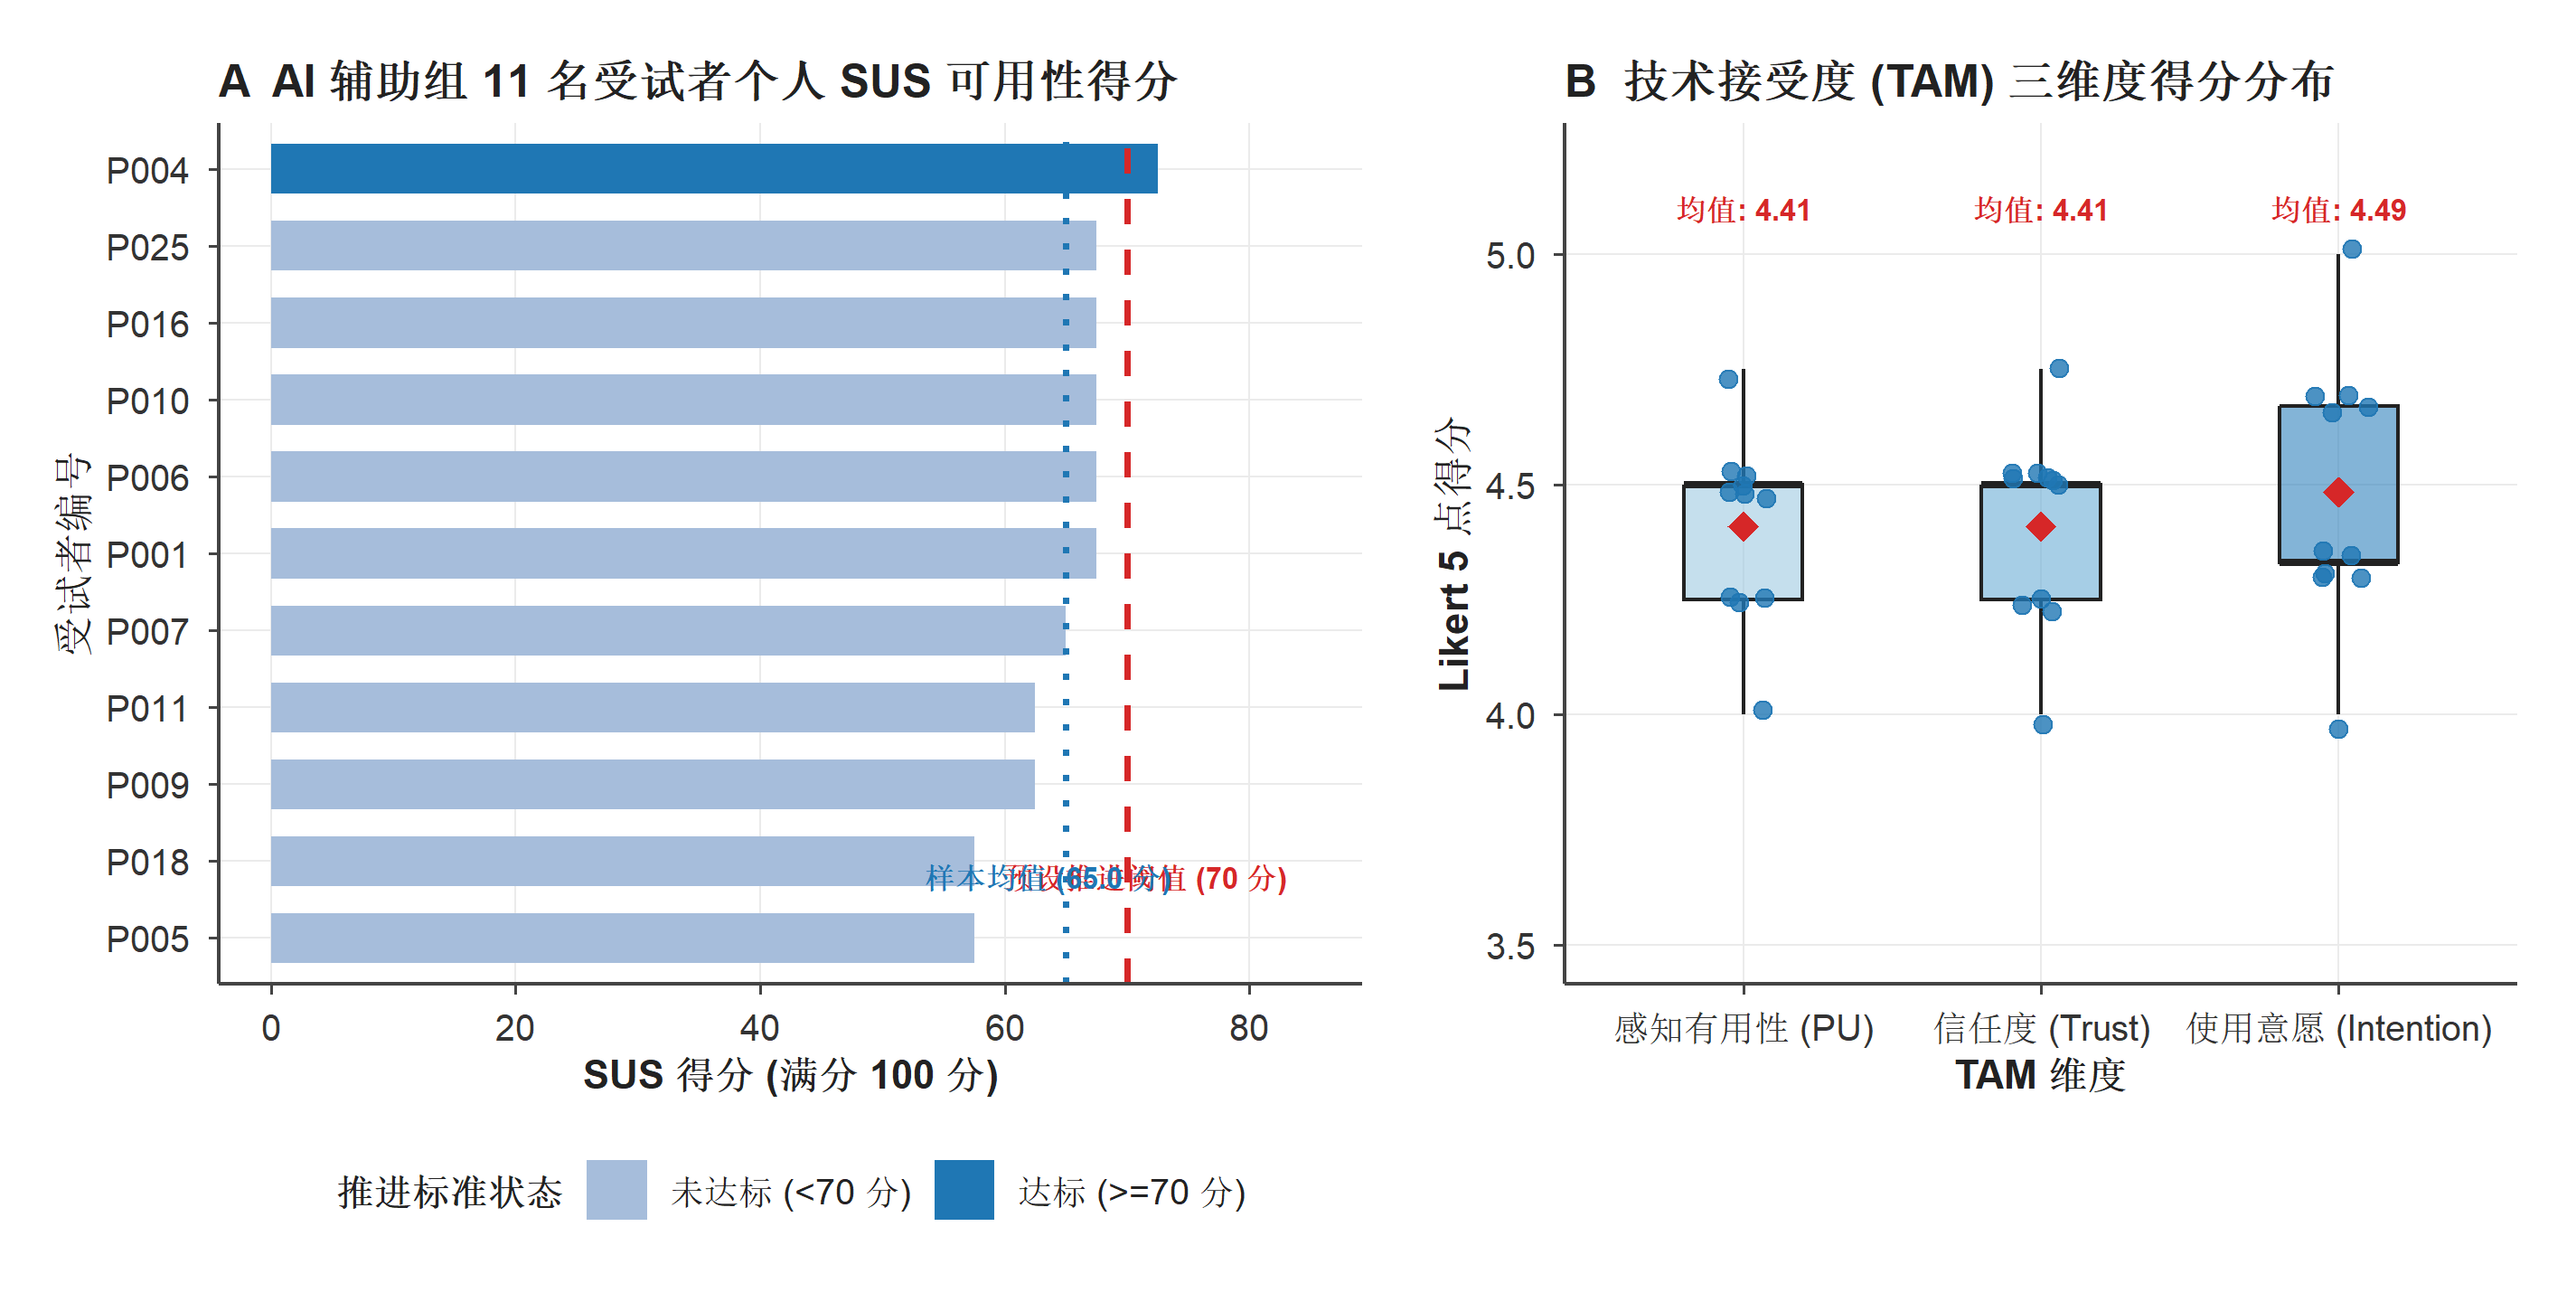
\includegraphics[width=0.95\textwidth]{figures/图4-5_系统评价与TAM接受度.png}
\caption{A：11名受试者个人SUS可用性得分，红色虚线为预设推进阈值（70分），蓝色点划线为样本均值（65.0分）；B：TAM三维度（感知有用性、信任度、使用意愿）Likert 5点得分箱线图，红星为均值}
\label{fig:sus_tam}
\end{figure}

\subsection{训练经验与工具需求差异}
\label{sec:experience_needs}

\textbf{主题五：训练经验和基线水平影响反馈需求。}

低力量或经验较少者更需要清晰的行动建议和外部安全边界；中高水平训练者更重视疲劳监测、训练精细化和自主权。系统不能假设所有训练者都需要同一种自动化程度。

P003、P027希望将速度或RIR转化为大白话行动建议；P010需要系统作为安全刹车；P012希望工具进行精准疲劳监测；P014希望系统进行赛后分析, 不希望实时指挥；P013希望使用设备验证自己的感觉；P018要求工具真正体现个体化和智能化。

该主题提示, 训练年限和基线力量可能是后续正式试验需要考虑的效应修饰因素, 但本研究样本量不足以进行正式交互检验。

\subsection{证据层面的分层理解}
\label{sec:evidence_layers}

\textbf{主题六：训练结果、系统评价和安全体验属于不同证据层面。}

访谈资料显示, 体能变化明显不一定带来较高系统评价, 系统评价较高也不一定意味着体能收益明显, 受试者认为安全和掌控感良好也不等于发生了客观伤病预防。

典型对照包括：P018的CMJ变化较明显（+10.30 cm），但SUS、PU、Trust和Intention相对较低；P016信任和有用性较高, 但体能变化有限；P015力量提高（1RM+17.50 kg）, 但SJ下降（-1.50 cm）；P013、P027力量和跳跃均有改善, 但机制仍不能由访谈单独确认。

该主题支持将研究结果分层理解：（1）工具测量层——App与GymAware一致性；（2）训练过程层——负荷执行与速度命中率；（3）体能适应层——1RM、CMJ、SJ变化；（4）心理接受层——SUS、PU、Trust、Intention评分。

\section{跨个案类型分析}
\label{sec:participant_types}

基于三轮主题分析, 研究三归纳出五类跨个案类型。个性化数智化监控的理论框架概念图见图~\ref{fig:framework}。

\begin{figure}[htbp]
\centering
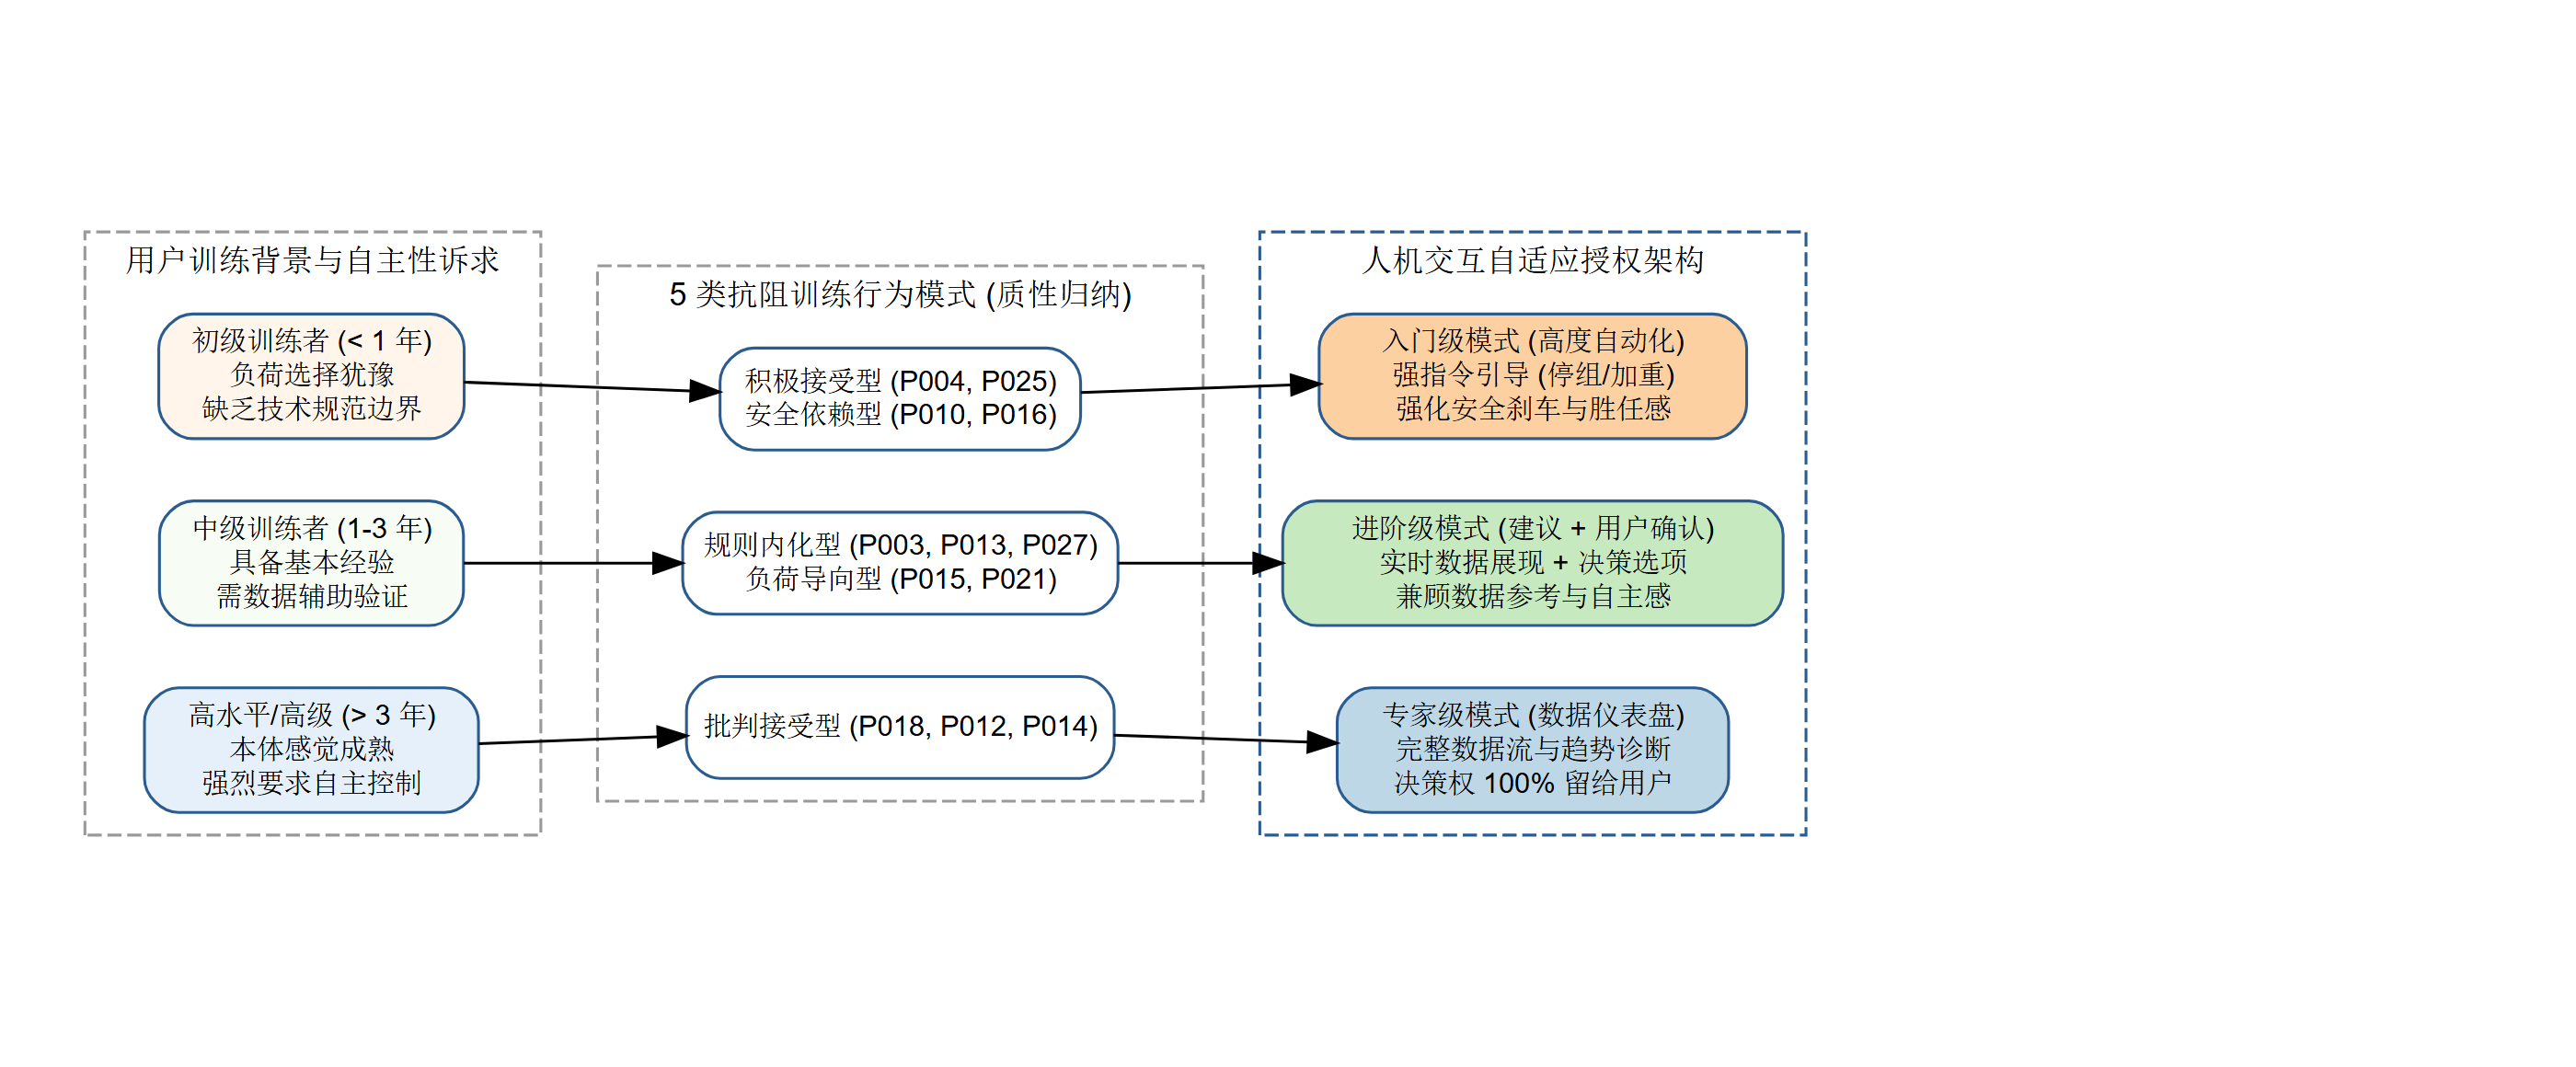
\includegraphics[width=0.95\textwidth]{figures/图4-7_分层匹配理论框架.png}
\caption{个性化数智化监控理论框架：用户训练背景决定行为模式，行为模式决定最优人机交互授权架构}
\label{fig:framework}
\end{figure}

\subsection{积极接受型}
代表受试者：P025、P004。

该类型特征包括：愿意执行系统建议；认可速度反馈的价值；愿意继续使用系统；关注加重、突破和流程效率。这类受试者将系统视为训练推进的辅助工具, 对系统的建议执行度较高。

\subsection{安全依赖型}
代表受试者：P010、P016。

该类型特征包括：主要关注受伤风险和疲劳；接受系统减量或停组；将系统视为外部安全边界；可能担心规则过于保守。这类受试者在安全感和训练刺激之间存在张力, 需要在保护与进取之间寻求平衡。

\subsection{批判性接受型}
代表受试者：P018、P012、P014。

该类型特征包括：承认工具或速度理念有价值；同时批评硬件、算法、解释或智能体验；强调训练者自主权；不接受系统替代身体判断。这类受试者对系统有较高期望, 当期望未满足时容易产生落差感。

\subsection{规则内化型（自我指导组）}
代表受试者：P003、P013、P027。

该类型特征包括：能把RIR转化为动作质量边界；能够进行自主减重、减次数或延长休息；自我效能来自掌控感和安全感；对速度反馈具有条件性需求。这类受试者在没有外部反馈的情况下仍能保持较好的自我调节能力。

\subsection{负荷导向型（自我指导组）}
代表受试者：P015、P021。

该类型特征包括：重视重量、次数或局部酸胀；容易接近力竭或采用慢速硬顶；力量增长不一定转化为爆发力；对速度反馈和外部停止边界有较强需求。这类受试者对内部感觉的依赖较强, 可能低估动作质量下降的风险。

\section{本章小结}
\label{sec:chapter_summary}

本章呈现了三个研究阶段的完整结果。

研究一在受控实验条件下验证了SportSci Pro与GymAware在杠铃后蹲MCV测量上的一致性。Rep级配对分析ICC=0.991, 热身级配对分析ICC=0.987, MAE分别为0.017和0.021 m/s, 一致性达到"优秀"水平。

研究二作为Pilot RCT, 共纳入24名受试者完成干预。主要发现包括：（1）可行性指标7/9达标, 主要后测完成率66.7\%和SUS评分65.0分未达标；（2）两组训练负荷总体相当, 自我指导组总重复次数略高（$p$=0.035）；（3）Hooper指数呈现显著课次主效应（$p$=0.004）, 组间差异不显著；（4）AI辅助组训练自我效能显著高于自我指导组（$p<0.001$, Hedges'$g$=2.70）；（5）CMJ高度调整后差值+2.16 cm, 接近但未达到统计显著性（$p$=0.051）。

研究三通过质性访谈揭示了训练者决策协商的深层机制。核心范畴为"客观反馈与自主判断之间的决策协商"。六大主题涵盖反馈决策价值、RIR动作质量边界、自动减组安全张力、系统接受多元维度、经验需求差异和证据分层理解。五类跨个案类型反映了个体在数智化监控环境下的差异化适应路径。
